%%%%%%%%%%%%%%%%%%%%%%%%%%%%%%%%%%%%%%%%%%%%%%%%%%%%%%%%%%%%%%%%%%%%%%%%%%%%%%%
%
% Tommy P. Keane
% Master of Science Thesis
% Department of Electrical and Microelectronic Engineering
% Rochester Institute of Technology
%
% April 2011
%
%
%
% Funded By: Lenel Systems Inc., A UTC Fire & Security Corporation
%
% Algorithm Intellectual Property Owned By: Lenel Systems Inc.
%
%
% http://www.tommypkeane.com
%
%%%%%%%%%%%%%%%%%%%%%%%%%%%%%%%%%%%%%%%%%%%%%%%%%%%%%%%%%%%%%%%%%%%%%%%%%%%%%%%

%%%%%%%%%%%%%%%%%%%%%%%%%%%%%%%%%%%%%%%%%%%%%%%%%%%%%%%%%%%%%%%%%%%%%%%%%%%%%%%
%
% CHAPTER 3
%
% SECTION 2: Feature Extraction
%
%%%%%%%%%%%%%%%%%%%%%%%%%%%%%%%%%%%%%%%%%%%%%%%%%%%%%%%%%%%%%%%%%%%%%%%%%%%%%%%


%%%%%%%%%%%%%%%%%%%%%%%%%%%%%%%%%%%%%%%%%%%%%%%%%%%%%%%%%%%%%%%%%%%%%%%%%%%%%%%
% BEGIN DOCUMENT

For the WFMI algorithm it was reasoned that the initial stage of feature extraction should be simple enough to allow the eventual possibility of real-time operation, but must still provide robust enough features to secure success in a variety of complex and unknown scenarios. Looking to the work in \cite{Ugarriza2009} the choice of color gradient features was found appropriate to provide a robust set of non-rigid shape details that, even under scaling and quantization, preserve a significant amount of the original information from the color video frames. After generating the RGB-gradient map (which is a floating point single channel image) a quantization step was implemented to achieve a computationally efficient algorithm.

Given an $\mathfrak{m}\times\mathfrak{n}$ 8-bpp pair of 3-channel color images, each  image (typically $480\times640$) is first processed to extract a feature map. The algorithm from \cite{Lee1991} is a vector-space gradient operation calculated by using the vectorized color pixel values ($\mathfrak{p}\times1$ vectors) as locations in the current color space (\ie RGB in this implementation). Taking horizontal and vertical gradients along each channel in the intensity domain and then using those resultant gradient images as inputs to the calculation of the maximum eigenvalue of the color-space Jacobian provides an essentially infinite, floating-point range of intensity values in the resultant color gradient map (again: single channel). In a practical implementation, there is an earlier, intial quantization required to limit this theoretically infinite floating-point map to the bit-depth of data-type. In the MATLAB\textsuperscript{\textregistered} and OpenCV implementations this was set to 64-bits, and this is the maximum amount of information that can be generated or stored by these features. Any quantization operation beyond this will superfluously remove information, but will enhance computational efficiency in the PMF calculation which has a range of $2^{b}$ (with $b$ being the bit-depth) maximum bins; so the key is to then discern what amount of quantization will maintain enough information to generate an appropriate and accurate mutual information map that is applicable for further processing in the registration search.

In order to determine the appropriate amount of quantization it is necessary to look ahead to the next step of the algorithm. The subsequent step of the algorithm is to perform an affine transform search with an exhaustive translation search. This will be explained in Section 3.3, but in order to perform a computationally efficient search with a metric based on joint and marginal PMF calculations for each translation in the exhaustive search, there is a need to quantize the color gradient maps into the ``edge'' maps. This secondary quantization results in maps on the order of one to four bits of pixel depth (still single channel) thus providing on the order of 3 to 30 distinct ``edges''. Since the PMF calculations will be based on full range histograms, as was discussed, then the joint PMF size will be $2^{b_{e}}\cdot2^{b_{e}}$, where $b_{e}$ is the bit-depth of the gradient to ``edge'' quantization. (Note: the use of ``edge'' is to maintain that this is not a binary map, there is no thresholding operation, the gradient is simply quantized so a syntactical distinction is being made.)

\begin{figure}[h]
\centering
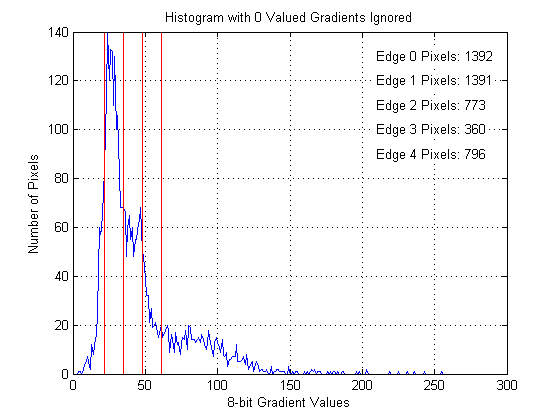
\includegraphics[width=.8\textwidth]{GradientHistogram}
\caption{Example Gradient Map Histogram with Quantization Boundaries}
\label{gradienthistogram}
\end{figure}

The stronger the quantization, \ie{ }the fewer the number of ``edges'', the less information available in the image from the color-space gradient map, yet this is inversely proportional to the computational efficiency. Also, discussed in more detail later on, in the use of a hierarchical search there is an added concern as to the effects of the subsampling on the image information. These are all significant implementation concerns, and it was found that the fastest and most accurate implementation was achieved with $b_{e}=2$, thus having 4 significant ``edges'' while zero values were ignored in the PMF calculations. To determine the quantization a simplification of the method in \cite{Ugarriza2009} was used where the gradient map histogram was quantized. The top 20\% of the pixels were empirically determined as the strong object ``edges'', with the bottom 10\% being determined as noise or superfluous detail ``edges''. The remaining 70\% of the pixels were evenly split into $b_{e}-1$ groups of so-called significant detail ``edges''. As the gradient histogram was found to typically follow a low-variance poission-like distribution with right skew, these percentage bounds were found to empirically average the distribution rise with the bottom 10\%, the long tail with the top 20\%, and the majority of the distribution with the middle 70\%. This was an empirical development that is fast, efficient, and has been found to provide useful and conceptually valid ``edges'' in the realistic test images. A visualization of this quantization is shown in Figure \ref{gradienthistogram}.


%%%%%%%%%%%%%%%%%%%%%%%%%%%%%%%%%%%%%%%%%%%%%%%%%%%%%%%%%%%%%%%%%%%%%%%%%%%%%%%
% END OF DOCUMENT

